\chapter{Introduzione alla Materia Oscura}
\label{ch:materia_oscura}

Il concetto di materia oscura si riferisce a una componente ipotetica di materia che non emette, non assorbe e non riflette la radiazione elettromagnetica, risultando di fatto invisibile ai tradizionali strumenti di osservazione astronomica. La sua presenza viene dedotta esclusivamente attraverso gli effetti gravitazionali che essa esercita sulla materia visibile (o barionica) e sulla propagazione della luce su scale galattiche e cosmologiche.

L'esistenza di una componente di massa non luminosa nell'universo è stata postulata per la prima volta negli anni '30 del Novecento dall'astrofisico svizzero Fritz Zwicky, attraverso lo studio del moto delle galassie all'interno del \textit{Coma Cluster}. 
Negli anni '70, lo studio delle curve di rotazione delle galassie a spirale fornì una prova incontrovertibile dell'esistenza di materia oscura nell'universo.

Oggi, grazie ai precisi dati cosmologici ottenuti dai telescopi spaziali, sappiamo che la materia ordinaria costituisce solo una frazione minima del nostro Universo. All'interno del modello cosmologico standard ($\Lambda$CDM), la materia oscura costituisce circa il 26.8\% della densità di energia totale dell'universo (corrispondente a oltre l'80\% della materia totale esistente), mentre la materia barionica rappresenta appena il 4.9\%. Il restante 68.3\% è costituito dall'energia oscura, responsabile dell'espansione accelerata del cosmo.

Nel corso degli ultimi decenni, sono state raccolte numerose e indipendenti evidenze sperimentali a sostegno della presenza di materia oscura su diverse scale cosmiche. Oltre alle curve di rotazione galattiche, prove cruciali derivano dallo studio delle anisotropie della Radiazione Cosmica di Fondo (CMB), dall'effetto di lente gravitazionale osservato nei grandi ammassi, e dalla dinamica di sistemi in collisione come il celebre \textit{Bullet Cluster}. 

\section{Evidenze astrofisiche e cosmologiche}
\label{sec:evidenze}
\subsection{Curve di rotazione delle galassie a spirale}
\label{subsec:curve_rotazione}

Una delle evidenze più robuste e immediate della presenza di materia oscura su scala galattica deriva dallo studio delle curve di rotazione delle galassie a spirale. La curva di rotazione rappresenta l'andamento della velocità orbitale $v(r)$ delle stelle e del gas interstellare in funzione della loro distanza $r$ dal centro galattico.

Sperimentalmente, la determinazione delle velocità a grandi distanze dal nucleo è resa possibile dall'osservazione dello spostamento Doppler (redshift e blueshift) della riga di emissione a \SI{21}{\cm} dell'idrogeno neutro. Esso rappresenta un ottimo tracciante cinematico poiché le nubi di idrogeno neutro si estendono molto al di fuori del disco visibile della galassia, permettendo di raccogliere dati anche a molti kiloparsec di distanza dal centro galattico.

Dal punto di vista teorico, assumendo che la massa della galassia sia concentrata prevalentemente nella sua componente luminosa (stelle e gas) all'interno del bulge centrale e del disco, per regioni sufficientemente distanti dal centro ($r > R_{\mm{gal}}$) la massa racchiusa $M(r)$ approssima la massa totale visibile $M_{\mm{tot}}$ e diventa costante. Uguagliando la forza gravitazionale e la forza centripeta

\begin{equation}
\frac{G M(r) m}{r^2} = \frac{m v^2(r)}{r}
\label{eq:equilibrio_centripeto}
\end{equation}

ed esplicitando la velocità orbitale, si ottiene il profilo kepleriano atteso:

\begin{equation}
v(r) = \sqrt{\frac{G M(r)}{r}} \propto \frac{1}{\sqrt{r}}
\label{eq:andamento_kepleriano}
\end{equation}

Ci si aspetterebbe quindi una curva che, dopo una crescita iniziale lineare nel core galattico e il raggiungimento di un picco, decada proporzionalmente a $1/\sqrt{r}$ all'aumentare della distanza.

\begin{figure}[htbp]
\centering
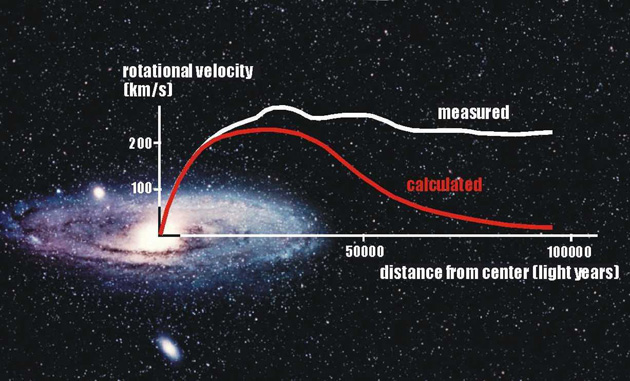
\includegraphics[width=0.6\linewidth,angle=0]{figures/curva_di_rotazione.jpg}
\caption{Confronto tra la curva di rotazione predetta dal modello kepleriano (in rosso) basato sulla sola materia visibile e la curva osservata sperimentalmente (in bianco), caratterizzata da un andamento piatto.}
\label{fig:curva_rotazione}
\end{figure}

Tuttavia, le osservazioni cinematiche mostrano un andamento radicalmente differente: superato il picco iniziale, la curva di rotazione non decade affatto, ma rimane approssimativamente costante a un valore $v_{\mm{max}}$ costante fino a diverse decine di kiloparsec dal centro, come mostrato in Figura \ref{fig:curva_rotazione}.

Per mantenere $v(r) = \text{costante}$ nell'equazione \eqref{eq:andamento_kepleriano}, la massa totale racchiusa non può essere costante, ma deve crescere linearmente con il raggio:
\begin{equation}
M(r) \propto r
\end{equation}
Questo comportamento implica necessariamente la presenza di una considerevole componente di massa non luminosa che domina le regioni esterne della galassia, il cui profilo di densità deve decadere come il quadrato del raggio:
\begin{equation}
\rho(r) \propto \frac{1}{r^2}
\end{equation}
Tale distribuzione di densità è incompatibile con la struttura geometrica a disco tipica della materia barionica visibile in queste galassie. Inoltre, lo studio della cinematica stellare perpendicolare al piano galattico (ovvero le misurazioni effettuate sul moto verticale delle stelle) conferma che questo deficit di massa non è confinato sul piano del disco, ma è distribuito in modo isotropo e sfericamente simmetrico. Si teorizza quindi che ogni galassia a spirale sia immersa in un vasto e massiccio alone di materia oscura a simmetria sferica, che si estende ben oltre i confini della materia visibile.

\subsection{Il Bullet Cluster e gravitational lensing}
\label{subsec:bullet_cluster}

\begin{figure}[htbp]
\centering
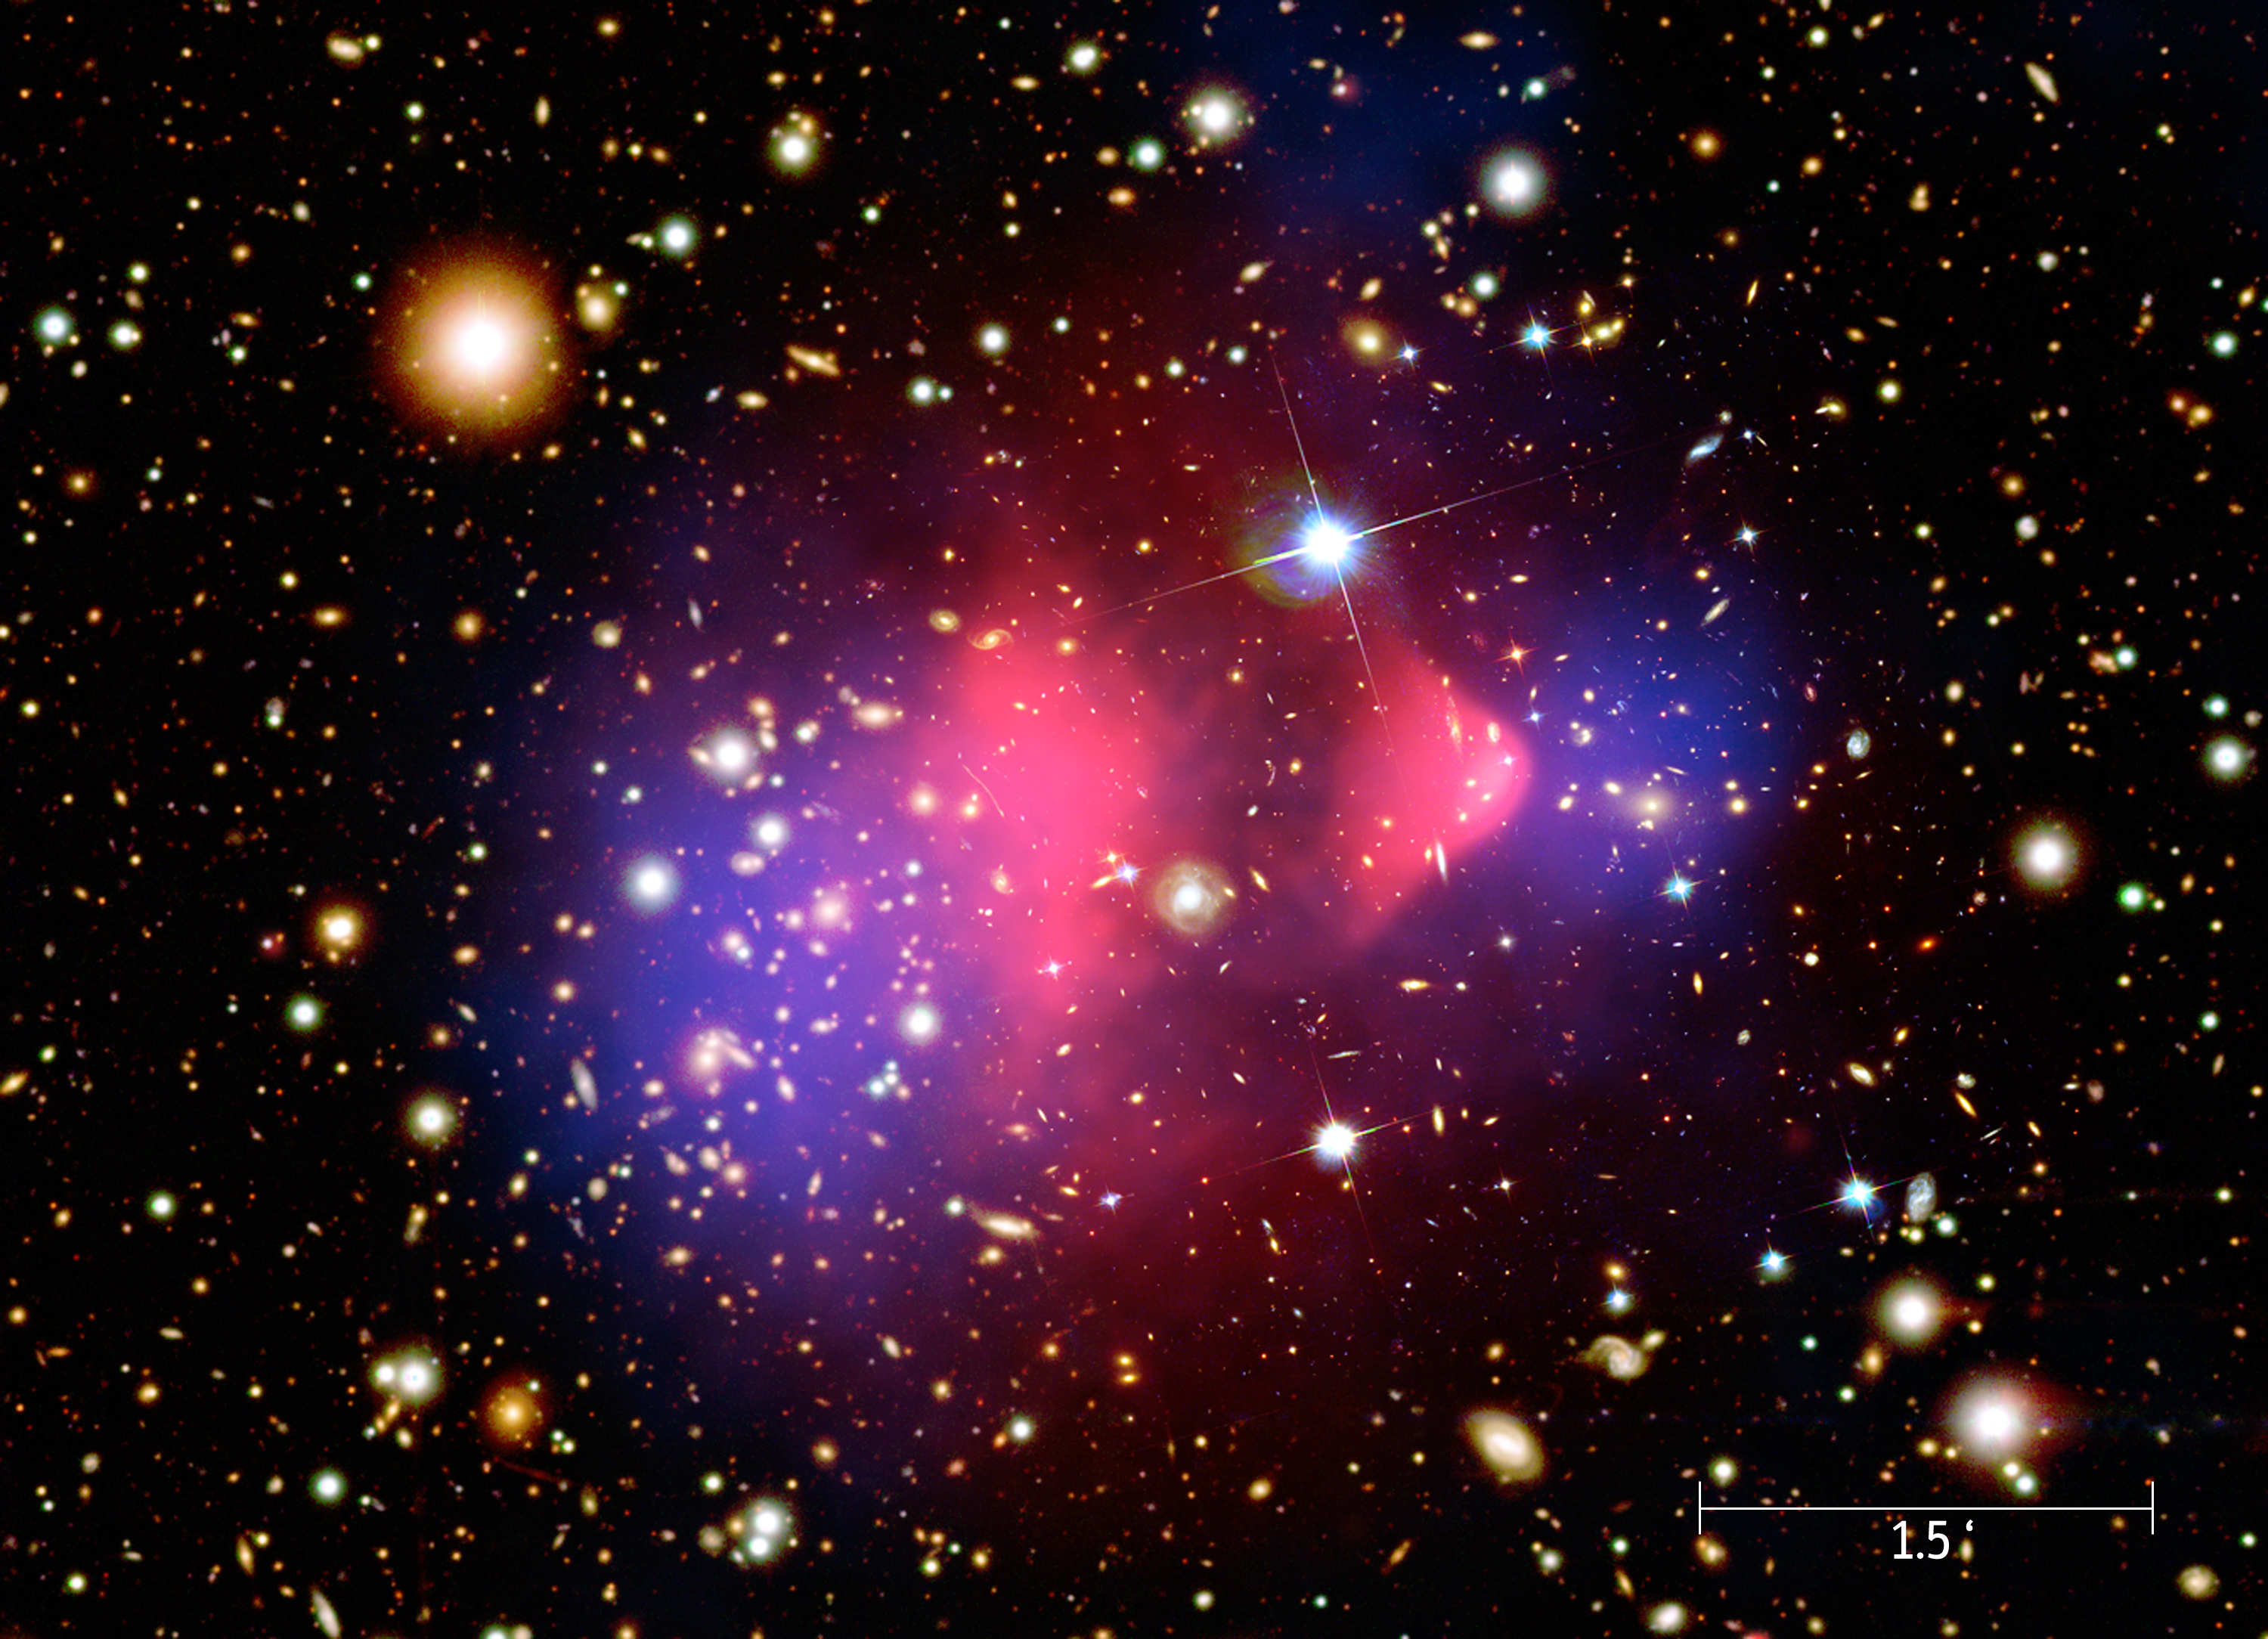
\includegraphics[width=0.6\linewidth,angle=0]{figures/bullet_cluster.jpg}
\caption{Bullet Custer: in rosa il gas intracluster che emette raggi X, in blu la distribuzione di materia oscura calcolata tramite \textit{gravitational lensing}. Sullo sfondo la stessa immagine vista nello spettro ottico. Immagine presa da \cite{chandra_bullet_2006}}
\label{fig:bullet_cluster}
\end{figure}

Un'altra convincente prova dell'esistenza di materia oscura, proviene dallo studio dell'ammasso di galassie \textit{Bullet Cluster} (1E 0657-558). Questo sistema è il risultato di una collisione ad alta velocità tra due sotto-ammassi di galassie.

In un ammasso galattico, la componente barionica dominante in termini di massa non è rappresentata dalle stelle delle galassie, bensì dal gas interstellare caldo, detto \textit{Intracluster medium} (ICM), che permea lo spazio tra una galassia e l'altra. Durante la collisione, la materia barionica ha manifestato comportamenti macroscopicamente distinti:
\begin{itemize}
    \item \textbf{Il gas intra-ammasso}, interagendo attraverso interazione elettromagnetica, ha subito un forte attrito che ne ha causato il rallentamento e il conseguente riscaldamento, lasciandolo confinato nella regione centrale dello scontro, dove si nota una forte emissione di raggi X termici di frenamento (\textit{bremsstrahlung}).
    \item \textbf{Le componenti stellari} delle galassie, essendo sistemi compatti, sono passate oltre la zona di impatto senza subire rallentamenti significativi.
\end{itemize}

Se la dinamica cosmologica fosse governata esclusivamente dalla materia barionica soggetta a leggi gravitazionali modificate (come la teoria MOND, \textit{Modified Newtonian Dynamics}, che cerca di giustificare l'andamento della curva di rotazione delle galassie a spirale senza introdurre la materia oscura), il minimo del potenziale gravitazionale del sistema dovrebbe coincidere con il centro della distribuzione spaziale del gas, dove risiede la quasi totalità della massa ordinaria.

Tuttavia, le mappe della densità di massa totale ottenute mediante tecniche di \textit{gravitational lensing}, sfruttando le distorsioni geometriche della luce proveniente da galassie di fondo, mostrano che i minimi del potenziale gravitazionale si trovano in corrispondenza delle componenti galattiche che non hanno subito collisioni, nettamente separati e spazialmente disaccoppiati dal plasma barionico, come visibile in Figura \ref{fig:bullet_cluster}.

Questo fenomeno di disaccoppiamento spaziale tra la massa visibile e il centro di massa gravitazionale fornisce la prova empirica che la maggior parte della materia nel sistema è costituita da una componente invisibile che sicuramente non interagisce nè tramite interazione elettromagnetica nè forte: la materia oscura.


\subsection{Anisotropie della Radiazione Cosmica di Fondo (CMB)}
\label{subsec:cmb}

Mentre le curve di rotazione galattiche e il Bullet Cluster costituiscono evidenze di natura astrofisica e locale, la Radiazione Cosmica di Fondo (CMB, \textit{Cosmic Microwave Background}) fornisce una prova di natura prettamente cosmologica, legata all'evoluzione dell'Universo primordiale. 

La CMB rappresenta la radiazione fossile emessa all'epoca della ricombinazione (circa $380\,000$ anni dopo il Big Bang), quando la temperatura del cosmo discese sotto la soglia dei $\sim 3000\text{ K}$. A queste energie, i protoni e gli elettroni liberi si legarono per formare idrogeno neutro; questo evento causò il disaccoppiamento dei fotoni dal plasma barionico, rendendo l'Universo trasparente alla radiazione. I fotoni primordiali, in viaggio da allora, hanno subito un drastico redshift a causa dell'espansione cosmologica fino a raggiungere i nostri rivelatori.

La mappa della CMB (Figura \ref{fig:CMB}) mostra uno spettro di corpo nero quasi perfetto a una temperatura media di $T_0 \approx 2.725\text{ K}$, caratterizzato da microscopiche fluttuazioni termiche dell'ordine di $\Delta T / T_0 \sim 10^{-5}$. Dal punto di vista fisico, tali fluttuazioni (chiamate anisotropie della CMB) rappresentano la firma termica delle onde acustiche primordiali: esse costituiscono i "semi" da cui si sono formate le attuali strutture cosmiche, come galassie e ammassi, e offrono una prova decisiva della presenza di materia oscura.

Nel plasma antecedente alla ricombinazione, la materia barionica era soggetta a due forze contrapposte: l'attrazione gravitazionale, che ne favoriva il collasso, e la pressione di radiazione esercitata dai fotoni (fortemente accoppiati agli elettroni tramite \textit{scattering Thomson}), che tendeva a far espandere il fluido verso l'esterno. Questa competizione generava delle vere e proprie oscillazioni acustiche.

In questo scenario, il ruolo della materia oscura risulta fondamentale. Essendo priva di accoppiamento elettromagnetico, la materia oscura non risentiva della pressione di radiazione dei fotoni. Di conseguenza, ha potuto iniziare il proprio collasso gravitazionale molto prima della ricombinazione, scavando pozzi di potenziale gravitazionale profondi e stabili all'interno dei quali la materia barionica è successivamente precipitata.

L'analisi statistica di queste anisotropie viene eseguita scomponendo la mappa in armoniche sferiche per ricavarne lo spettro di potenza angolare (Figura \ref{fig:PowerSpectrum}). L'altezza e la posizione dei picchi acustici di questo spettro forniscono una misura diretta e ad altissima precisione dei parametri cosmologici. 

\begin{figure}[h]
\centering
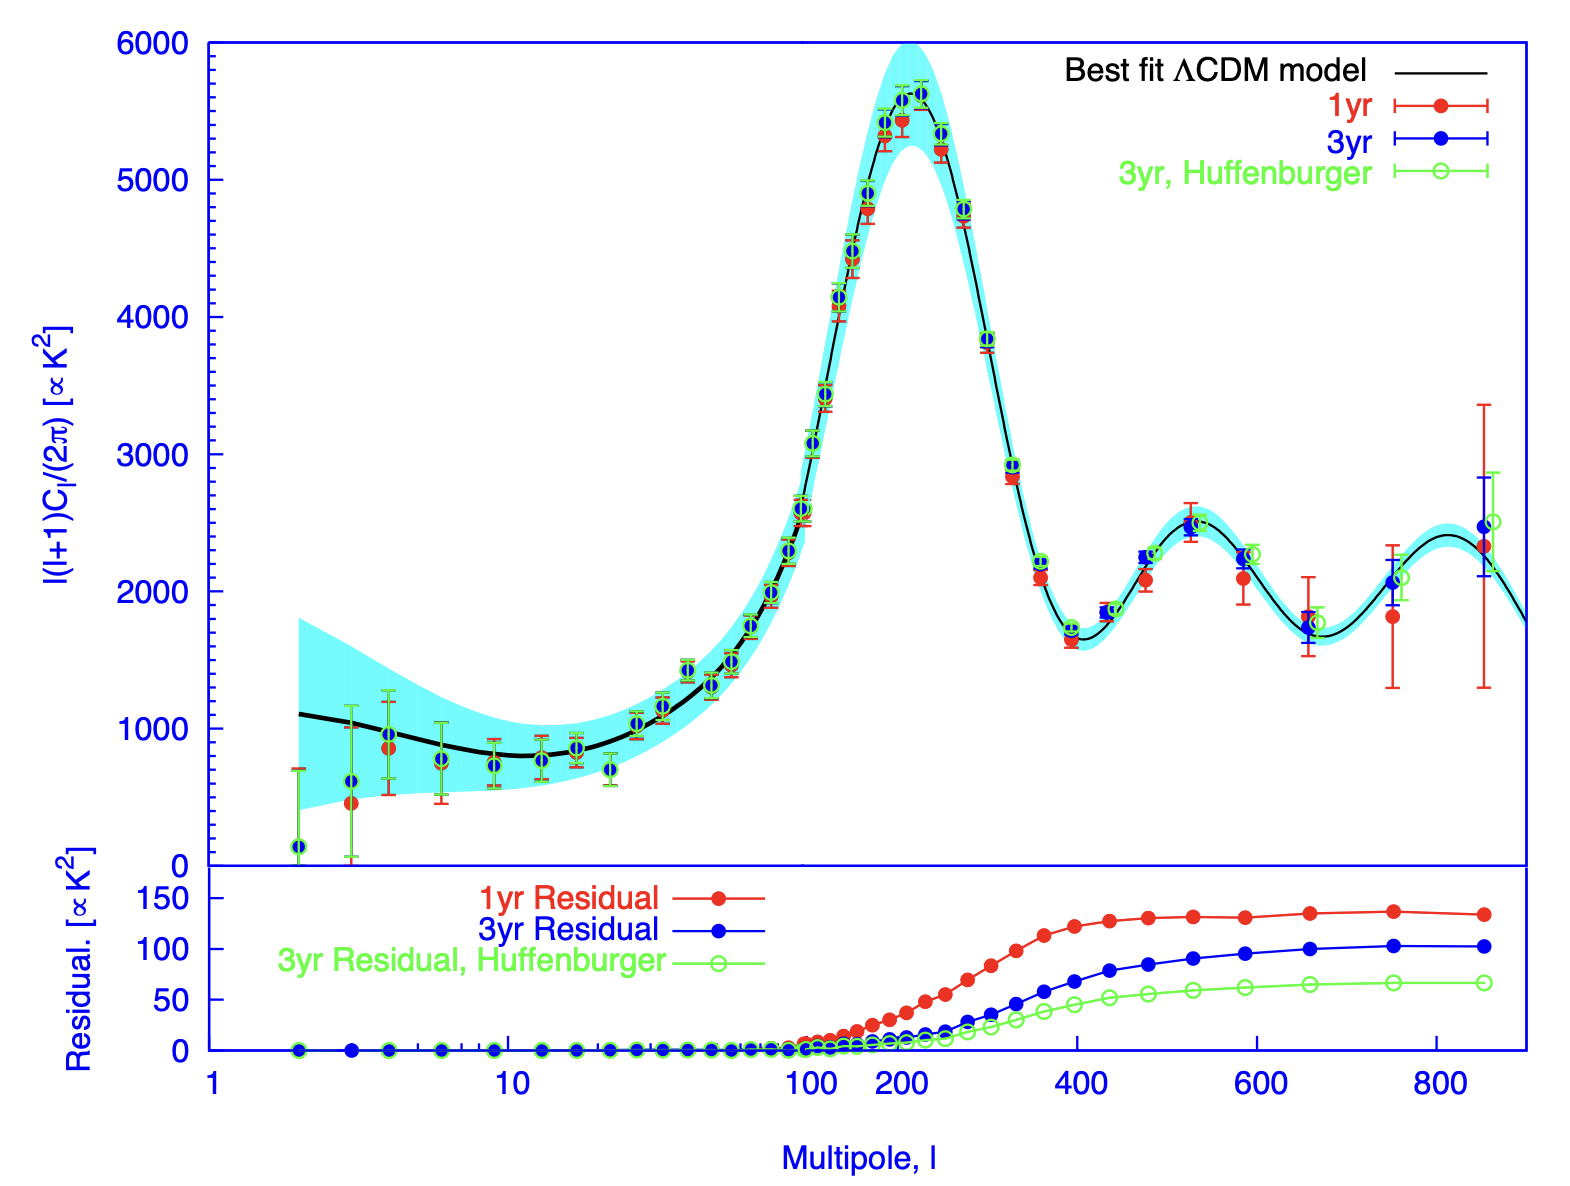
\includegraphics[width=0.6\linewidth]{figures/spettro_pot_ang.png}
\caption{Spettro di potenza angolare ottenuto da WMAP-1 (rosso) e WMAP-3 (blu) confrontato con la previsione teorica del modello $\Lambda$CDM (linea nera). L'asse delle ascisse rappresenta il momento di multipolo $\ell$, mentre l'asse delle ordinate mostra l'ampiezza delle anisotropie della CMB. Immagine tratta da \cite{Souradeep2006AngularPS}.}
\label{fig:PowerSpectrum}
\end{figure}

Il primo picco, situato a una scala angolare $\theta \approx 1^\circ$ (corrispondente al momento di multipolo $\ell \approx 220$), rappresenta l'ampiezza apparente delle regioni di plasma che hanno fatto in tempo a subire esattamente una sola massima compressione prima del disaccoppiamento. La sua posizione fornisce la prova sperimentale che l'Universo è geometricamente piatto ($\Omega = 1$).

L'evidenza più marcata della materia oscura emerge dall'analisi dei picchi successivi. Il secondo picco, corrispondente alla prima fase di massima rarefazione (il "rimbalzo" del plasma verso l'esterno), risulta significativamente più basso rispetto al primo. Questo smorzamento è dovuto proprio all'azione della materia oscura: non subendo la spinta della radiazione, la materia oscura è rimasta confinata nel fondo dei pozzi di potenziale, esercitando una forte attrazione gravitazionale che ha ostacolato e frenato l'espansione del fluido barionico verso l'esterno. Il terzo picco, legato alla seconda compressione massima, beneficia nuovamente del potenziale gravitazionale della materia oscura, mostrando un'ampiezza paragonabile al secondo picco.

I dati sperimentali confermano con straordinaria precisione il modello cosmologico standard $\Lambda\text{CDM}$, stabilendo che la materia oscura fredda (CDM) costituisce circa il $26.8\%$ della densità di energia totale dell'Universo, a fronte di un esiguo $4.9\%$ attribuibile alla materia barionica ordinaria.

\begin{figure}[htbp]
\centering
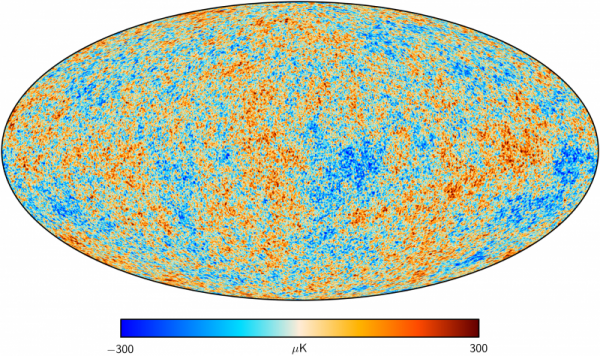
\includegraphics[width=0.6\linewidth]{figures/planck_int_cmb_0.png}
\caption{Mappa delle anisotropie di temperatura della radiazione cosmica di fondo ricostruita con i dati del satellite Planck. La CMB si comporta come un corpo nero con una temperatura media di $2.725\text{ K}$, presentando minime deviazioni da un emettitore perfetto. Tali deviazioni si manifestano come fluttuazioni termiche dell'ordine di circa $\pm 300\ \mu\text{K}$ (con variazioni medie di circa $18\ \mu\text{K}$), le quali riflettono le anisotropie primordiali della densità di materia. Immagine tratta da \cite{Planck2018Overview}.}
\label{fig:CMB}
\end{figure}

\section{Possibili candidati di Materia Oscura}
\label{sec:candidati}

Le evidenze cinematiche e cosmologiche discusse nei paragrafi precedenti delineano l'esistenza di una nuova forma di materia la cui natura fondamentale resta ignota, ma di cui è possibile tracciare un preciso profilo identitario. Affinché un candidato particellare sia accettabile, deve soddisfare simultaneamente quattro requisiti fondamentali:
\begin{enumerate}
    \item \textbf{Massivo:} dati gli effetti gravitazionali sulle galassie a spirale
    \item \textbf{Stabile o quasi-stabile:} con un tempo di vita medio nettamente superiore all'età dell'Universo ($\tau \gg 13.8 \times 10^9 \text{ anni}$), garantendone la permanenza dall'epoca della ricombinazione fino all'Universo locale contemporaneo.
    \item \textbf{Non luminoso:} elettricamente neutro e privo di carica di colore, per giustificare l'assenza di interazioni elettromagnetiche e forti dirette.
    \item \textbf{Non relativistico:} per permettere il corretto collasso gravitazionale delle strutture su piccola scala.
\end{enumerate}

I candidati di natura barionica non luminosa, storicamente raggruppati sotto il nome di MACHOs (\textit{Massive Compact Halo Objects}), sono oggi sperimentalmente esclusi dai dati ottenuti attraverso \textit{microlensing}. Si rende quindi necessario esplorare scenari di materia oscura non barionica.

Per catalogare la vasta gamma di particelle ipotizzate dalla fisica teorica, una prima fondamentale distinzione risiede nella cinematica delle particelle e nel loro impatto sulla formazione delle strutture:
\begin{itemize}
    \item \textbf{Hot Dark Matter (HDM):} Costituita da particelle leggere (scala dell'eV) e relativistiche. Avendo un'energia cinetica così elevata, è molto probabile si siano formati prima i superammassi che poi si sono divisi in strutture più piccole. Il modello che spiega questa evoluzione è detto Top-Down ed è oggi escluso dalle osservazioni della struttura su grande scala dell'Universo.
    \item \textbf{Cold Dark Matter (CDM):} Composta da particelle massive o nate cinematicamente fredde, con velocità non relativistiche ($v \ll c$) già nelle prime fasi evolutive. Il modello evolutivo di tipo Bottom-Up predice invece la formazione iniziale di piccole strutture, poi aggregatesi in ammassi più grandi.
\end{itemize}

\begin{figure}[t]
\centering
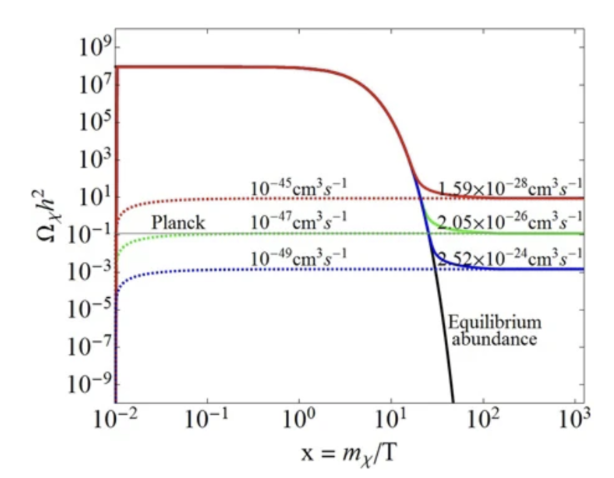
\includegraphics[width=0.6\linewidth,angle=0]{figures/freeze_in_out.png}
\caption{Confronto cinematico tra i meccanismi di produzione termica (\textit{freeze-out}, linee continue a destra) e non termica (\textit{freeze-in}, linee tratteggiate a sinistra) in funzione del parametro evolutivo $x = m_\chi / T$. La linea grigia orizzontale indica il valore della densità relitta misurato dal satellite Planck ($\Omega_{\chi} h^2 \approx 0.12$). Nel \textit{freeze-out}, le curve deviano dall'abbondanza di equilibrio termico a seconda della sezione d'urto di annichilazione. La linea verde, che fitta perfettamente i dati di Planck, corrisponde al valore ideale dell'interazione debole ($\sim 10^{-26} \text{ cm}^3\text{s}^{-1}$, il \textit{WIMP miracle}). Nel \textit{freeze-in}, l'abbondanza parte da zero e cresce per rari urti termici fino a stabilizzarsi; la linea verde tratteggiata rappresenta il valore di sezione d'urto di produzione necessario a riprodurre correttamente la densità di materia oscura attuale ($\sim 10^{-47} \text{ cm}^3\text{s}^{-1}$, impossibile da rilevare in esperimenti come CRESST). Immagine tratta da \cite{Chu2012DM}.}
\label{fig:freeze_in_out}
\end{figure}

Un secondo criterio di classificazione, riguarda il meccanismo di produzione della densità di materia oscura ($\Omega_{\mm{DM}}$) misurata oggi, illustrato in Figura \ref{fig:freeze_in_out}:
\begin{itemize}
    \item \textbf{Produzione Termica:} La materia oscura si trovava inizialmente in equilibrio termico e chimico con il plasma del Modello Standard nell'Universo primordiale, attraverso interazioni della forma
    \begin{equation}
        \text{DM$\,$+$\,$DM$\,$(+$\,$DM...)}\leftrightarrow \text{SM particles}.
    \end{equation} 
    La sua abbondanza attuale viene determinata dal meccanismo di \textit{freeze-out}, ovvero lo spegnimento delle reazioni di annichilazione dovuto all'espansione del cosmo.
    
    \item \textbf{Produzione Non Termica:} La materia oscura non termica non raggiunge l'equilibrio con le particelle del Modello Standard nel plasma primordiale, poiché governata da un'interazione estremamente più debole di quella nucleare debole. Viene generata per via quantistica o geometrica (come nei meccanismi di \textit{freeze-in} o di disallineamento), nascendo cinematicamente fredda anche se caratterizzata da una massa estremamente esigua.
\end{itemize}

I candidati più quotati al giorno d'oggi sono le WIMPs e gli assioni, entrambi appartenenti alla famiglia della Cold Dark Matter. Uno schema di tutti i possibili candidati in funzione della massa è riportato in Figura \ref{fig:candidati}

\begin{figure}[htbp]
\centering
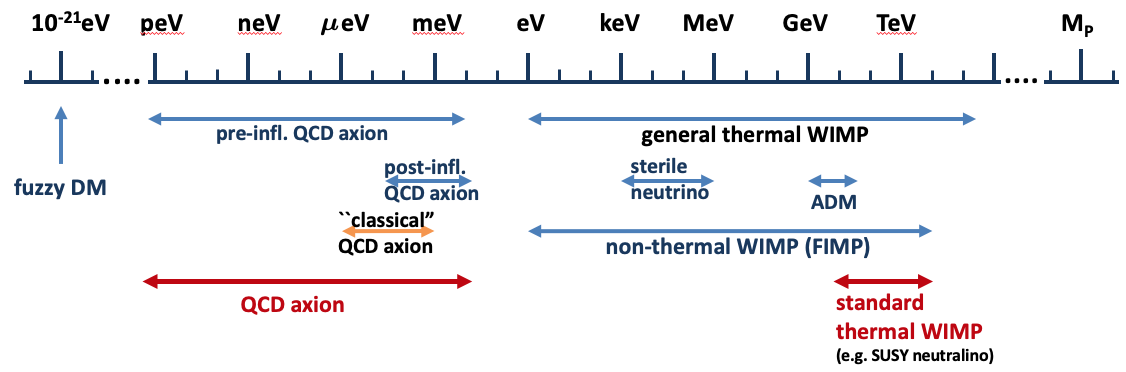
\includegraphics[width=1\linewidth,angle=0]{figures/dmmassrange_appecdmddreport_2020_v102.png}
\caption{Principali candidati di materia oscura divisi in range di massa, dal peV (assioni) alla massa di Planck ($1.2\cdot10^{19} \, \text{GeV}$)}
\label{fig:candidati}
\end{figure}

\subsection{WIMPs (Weakly Interacting Massive Particles)}
\label{subsec:wimps}

Le WIMPs rappresentano la classe di candidati di tipo CDM termico più accreditata e costituiscono l'obiettivo primario di esperimenti di rivelazione diretta come CRESST. Si tratta di particelle ipotetiche stabili, con una massa tipicamente compresa tra i $\mathrm{GeV}$ e i $\mathrm{TeV}$, che interagiscono con la materia ordinaria esclusivamente tramite la gravità e l'interazione nucleare debole (o un'interazione con sezione d'urto analoga).

Essendo candidati a produzione termica, nelle prime fasi dell'Universo queste particelle si trovavano in equilibrio chimico e termico con il plasma primordiale attraverso processi di creazione e annichilazione del tipo $\chi \bar{\chi} \rightleftharpoons \text{SM} \, \text{SM}$, in cui i due tassi di reazione si compensavano.

A seguito dell'espansione dell'Universo, la temperatura del plasma è scesa, e quando $ T < m_\chi$, il processo di creazione si è spento, mentre il processo di annichilazione, seppur rallentato dalla progressiva diluizione delle WIMP, è proseguito.

Quando il tasso di espansione dell'Universo ($H$) è diventato confrontabile e poi superiore al tasso di annichilazione, le particelle non sono più riuscite a incontrarsi efficacemente. Il processo di annichilazione si è congelato (\textit{freeze-out}) e l'abbondanza per unità di volume comovente ha determinato la densità relitta osservata oggi.

È interessante notare come le conclusioni teoriche ricavate inserendo i valori tipici della sezione d'urto dell'interazione debole conducano a una densità relitta che coincide sorprendentemente con i dati sperimentali osservati dal satellite Planck. Questa convergenza spontanea prende il nome di \textit{WIMP miracle}, e fornisce una solida giustificazione teorica alla ricerca di tali candidati nella finestra energetica dei $\mathrm{GeV}$-$\mathrm{TeV}$.

\subsection{Assioni}
\label{subsec:assioni}

L'assione è un candidato di materia oscura fredda a produzione non termica. La sua esistenza non è stata ipotizzata inizialmente per spiegare la massa mancante dell'Universo, ma per risolvere un problema teorico della fisica delle particelle noto come \textit{problema della CP forte}. Le equazioni della Cromodinamica Quantistica (QCD) permettono teoricamente una violazione della simmetria di Carica e Parità (CP) per le interazioni forti, che però non è mai stata osservata. 
Per giustificare ciò è stata ipotizzata una nuova simmetria globale, la cui rottura spontanea genera l'assione. Tramite questo meccanismo, il parametro che regola la violazione di CP viene guidato dinamicamente a zero.

La caratteristica principale dell'assione è la sua massa estremamente ridotta, che i modelli cosmologici attestano nella finestra dei micro-elettronvolt ($m_a \sim 10^{-6} - 10^{-3} \text{ eV}$).

Essendo particelle così leggere, si potrebbe erroneamente dedurre che gli assioni si muovano a velocità relativistiche, comportandosi come materia oscura calda. Tuttavia, queste particelle state generate da un processo detto meccanismo di disallineamento, che prevede la creazione di queste particelle a partire da oscillazioni del campo quantistico dell'assione, poiché esso si trovava disallineato rispetto al suo stato di minima energia. Queste oscillazioni si comportano come particelle con momento lineare quasi nullo, e dunque un candidato di CDM.

Dal punto di vista sperimentale, l'assione interagisce in modo talmente debole da non poter essere rivelato tramite gli urti nucleari cercati da esperimenti come CRESST. La ricerca di queste particelle avviene quindi tramite esperimenti radicalmente diversi dalla ricerca WIMP, basati sull'uso di speciali cavità risonanti note come aloscopi, che sfruttano la caratteristica degli assioni di convertirsi in fotoni (tipicamente nella frequenza delle microonde) quando attraversano un campo magnetico molto intenso.

\section{Tecniche di rivelazione}
\label{sec:rivelazione}

Rivelare la materia oscura rappresenta una delle sfide più complesse della fisica contemporanea, poiché l'unica interazione sperimentalmente accertata su scala macroscopica è quella di natura gravitazionale. Tuttavia, assumendo l'ipotesi che la materia oscura sia composta da WIMPs, si aprono tre possibili canali di indagine, basati sul potenziale accoppiamento con le particelle del Modello Standard.

\begin{itemize}
    \item \textbf{produzione nei collider}, in cui si tenta di produrre particelle di materia oscura facendo collidere particelle note ad altissime energie, cercandone la traccia sotto forma di energia o momento mancante nei prodotti di reazione.
    \item \textbf{rivelazione indiretta}, effettuata principalmente tramite telescopi terrestri e spaziali; questa tecnica mira a individuare i prodotti stabili derivanti dall'annichilazione o dal decadimento di particelle di materia oscura in zone ad alta densità cosmica (come il centro galattico), sotto forma di eccessi di raggi gamma, neutrini o antimateria.
    \item \textbf{rivelazione diretta}, consiste nell'esaminare in laboratori sotterranei gli urti elastici delle particelle di materia oscura del nostro alone galattico contro i nuclei atomici di un bersaglio (nel caso di CRESST, cristalli di $\text{CaWO}_4$).
\end{itemize}


I tre metodi di indagine sono riassunti schematicamente in Figura \ref{fig:schema_DM} e verranno analizzati singolarmente nei successivi paragrafi.

\begin{figure}[htbp]
\centering
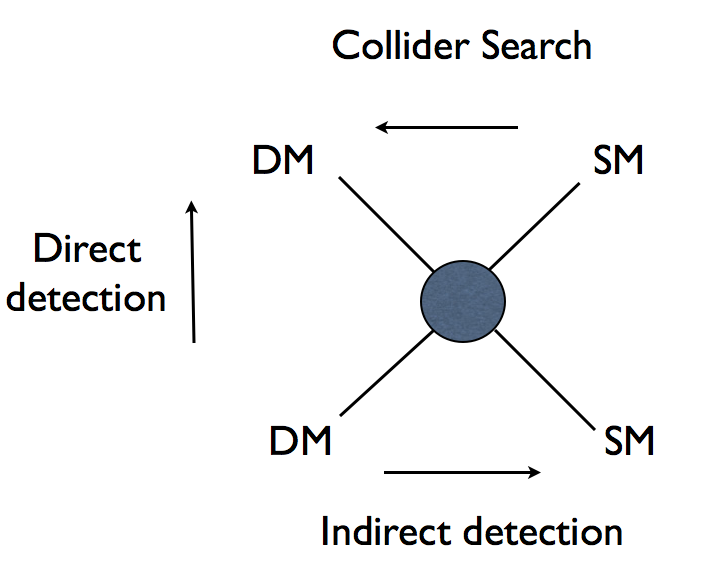
\includegraphics[width=0.5\linewidth,angle=0]{figures/scheme.png}
\caption{Rappresentazione schematica delle principali strategie di rivelazione della materia oscura.}
\label{fig:schema_DM}
\end{figure}

\subsection{Produzione nei collider}
La ricerca di materia oscura mediante collider viene svolta principalmente al \textit{Large Hadron Collider} (LHC), facendo scontrare particelle del Modello Standard ad alta energia e andando a cercare un deficit nel bilancio dell'energia o del momento totale delle particelle create. 

Tuttavia, trovare una nuova particella con questa tecnica non assicurerebbe automaticamente di aver individuato la materia oscura, ma si renderebbe necessaria una conferma indipendente tramite la rivelazione diretta o indiretta. Inoltre, date le brevi scale temporali e le distanze percorse dalle particelle all'interno dell'apparato sperimentale, non si avrebbe la certezza che la particella prodotta abbia una vita media paragonabile all'età dell'Universo, caratteristica invece fondamentale per la materia oscura.

\subsection{Rivelazione indiretta}
\label{subsec:indiretta}

Sebbene nel paragrafo \ref{subsec:wimps} si sia descritto il meccanismo di \textit{freeze-out} come il congelamento delle annichilazioni dovuto alla drastica diminuzione della densità di materia oscura nell'Universo, questo scenario assume un cosmo  omogeneo e non si applica su scala locale. All'interno delle strutture legate gravitazionalmente, come le galassie o gli ammassi di galassie, la materia oscura si è accumulata formando aloni ad altissima densità. In queste regioni, il tasso di interazione è sufficientemente elevato da consentire ai processi di annichilazione di proseguire attivamente anche nell'Universo contemporaneo.

La rivelazione indiretta si propone quindi di individuare i prodotti stabili derivanti da queste annichilazioni. Il processo genera particelle del Modello Standard che, attraverso successivi decadimenti, si convertono in flussi di raggi gamma, neutrini ad alta energia e antimateria cosmica (come antiprotoni e positroni). Questi segnali vengono successivamente catturati da telescopi e apparati sperimentali terrestri, come l'osservatorio per raggi gamma \textit{MAGIC} o il rivelatore di neutrini \textit{IceCube} al Polo Sud, oppure da spettrometri spaziali orbitanti a bordo della Stazione Spaziale Internazionale, come l'esperimento \textit{AMS-02}.

\subsection{Rivelazione diretta}
\label{subsec:rivelazione_diretta}

La rivelazione diretta tenta di catturare i rarissimi eventi in cui una WIMP appartenente all'alone di materia oscura attraversa un rivelatore posto in un laboratorio sotterraneo e subisce uno scattering elastico coerente contro il nucleo atomico di un materiale bersaglio.

\begin{figure} [b]
    \centering
    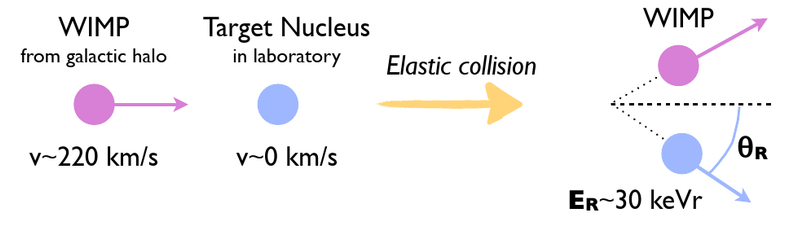
\includegraphics[width=0.6\linewidth]{figures/A-schematic-of-dark-matter-WIMP-elastic-scattering-off-a-target-nucleus.ppm.png}
    \caption{Scattering tra WIMP e nucleo target nel SR del laboratorio. In questo caso il massimo trasferimento di energia si avrebbe per $\theta_R = 0$}
    \label{fig:scattering}
\end{figure}

Il processo può essere modellizzato cinematicamente come un urto elastico a due corpi non relativistico (Figura \ref{fig:scattering}) tra una particella di materia oscura $\chi$ di massa $m_\chi$ e un nucleo a riposo di massa $m_N$. Nell'approssimazione in cui la WIMP possiede una velocità iniziale $v$ tipica del profilo galattico ($v \approx 220\,\mm{km/s}$), l'energia di rinculo $E_R$ trasferita al nucleo a seguito dell'impatto dipende dall'angolo di scattering $\theta$ nel sistema del centro di massa ed è espressa dalla relazione:

\begin{equation}
E_R = \frac{\mu_N^2 v^2}{m_N} (1 - \cos\theta)
\label{eq:energia_rinculo}
\end{equation}

dove $\mu_N$ rappresenta la massa ridotta del sistema WIMP-nucleo, definita come:

\begin{equation}
\mu_N = \frac{m_\chi m_N}{m_\chi + m_N}
\label{eq:massa_ridotta}
\end{equation}

Dall'equazione \ref{eq:energia_rinculo} si deduce che l'energia massima trasferita ($E_{\mm{max}}$) si ottiene nel caso $\theta = \pi$:

\begin{equation}
E_{\mm{max}} = \frac{2 \mu_N^2 v^2}{m_N}
\label{eq:energia_massima}
\end{equation}

Considerando i valori tipici previsti per le WIMP ($m_\chi \sim 100\,\mm{GeV}$) e le masse dei nuclei comunemente impiegati nei rivelatori (come l'Ossigeno, il Calcio o il Tungsteno nel caso dei cristalli di $\mm{CaWO}_4$ di CRESST), l'energia di rinculo risulta confinata in un range molto basso, tipicamente compresa tra frazioni di $\mm{keV}$ e poche decine di $\mm{keV}$. La difficoltà della rivelazione diretta consiste proprio nello sviluppare esperimenti che abbiano una sensibilità tale da poter misurare rilasci di energia così esigui.

\begin{figure}[htbp]
    \centering
    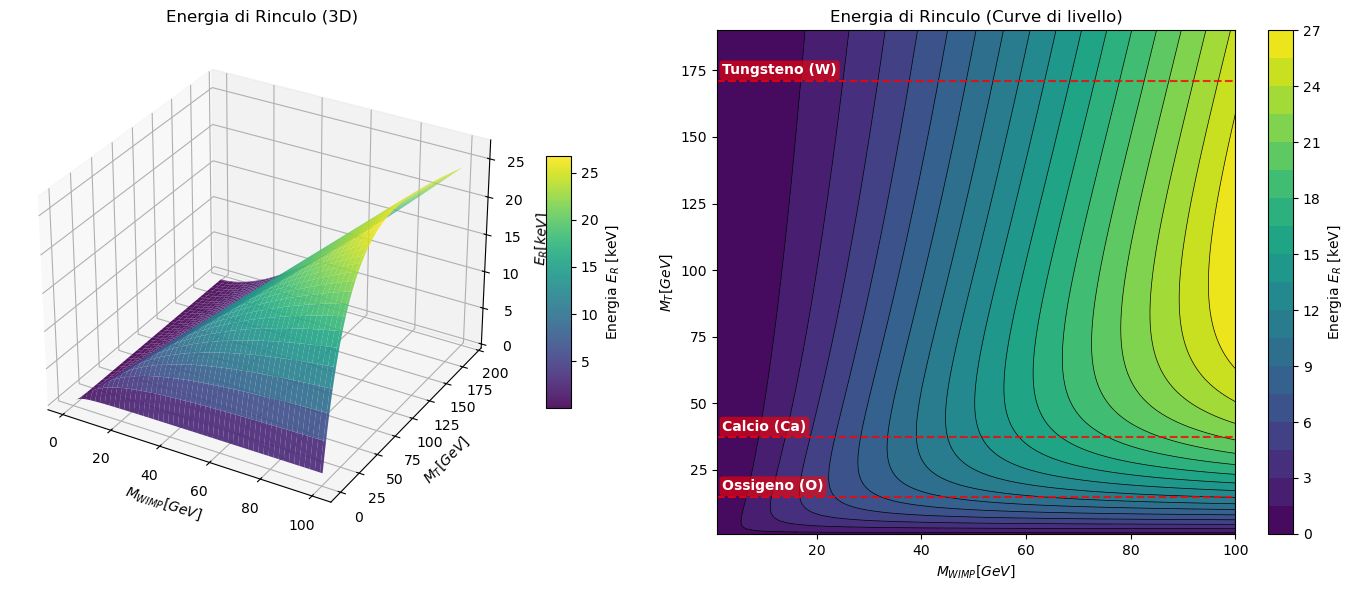
\includegraphics[width=1\linewidth]{figures/Energia_rinculo.png}
    \caption{Energia di rinculo (\ref{eq:energia_massima}) in funzione della massa della WIMP ($M_{WIMP}$) e della massa del nucleo bersaglio ($M_T$). A sinistra è mostrato l'andamento tridimensionale della funzione, mentre a destra è riportato il grafico a curve di livello, dove le linee tratteggiate rosse indicano le masse dei target di Ossigeno, Calcio e Tungsteno. Si nota come il trasferimento di energia sia massimo nel caso $M_{WIMP} \approx M_T$. Per questo motivo l'esperimento CRESST utilizza 3 bersagli con massa diversa, in modo da massimizzare la sensibilità su un ampio spettro di masse della materia oscura.}
    \label{fig:Energia_rinculo}
\end{figure}

\subsubsection{Tasso di eventi e sezione d'urto}
\label{subsec:rate_sezionedurto}
Il tasso di eventi stima quanti urti ci si aspetta di osservare in un intervallo di tempo e si esprime in numero di interazioni per unità di tempo e massa del rivelatore. La formula semplificata, che suppone la velocità delle particelle di materia oscura nell'alone $v$ costante è data da:

\begin{equation}
R = \frac{\rho_0}{m_\chi} \frac{\sigma_0}{m_N} v
\label{eq:rate_semplice}
\end{equation}
dove $\rho_0$ è la densità locale di materia oscura (stimata a circa $0.3\,\mm{GeV/cm}^3$), $m_\chi$ è la massa della WIMP, $m_N$ è la massa del nucleo bersaglio del rivelatore e $\sigma_0$ la sezione d'urto di scattering tra la WIMP e il nucleo

Nella realtà sperimentale, le particelle di materia oscura non viaggiano tutte alla stessa velocità, ma seguono una distribuzione statistica all'interno dell'alone galattico. Per questa ragione, l'espressione completa del tasso differenziale di eventi è data da:

\begin{equation}
\frac{\dd R}{\dd E_R} = \frac{\rho_0}{m_\chi m_N} \int_{v_{\mm{min}}}^{v_{\mm{fuga}}} v \cdot f(\vec{v}) \frac{\dd\sigma}{\dd E_R} \, \dd^3 v
\label{eq:rate_differenziale}
\end{equation}
dove $f(\vec{v})$ è la funzione di distribuzione delle velocità delle WIMP nel sistema di riferimento della Terra, $\frac{\dd\sigma}{\dd E_R}$ è la sezione d'urto differenziale di scattering, mentre $v_{\mm{min}}$ e $v_{\mm{esc}}$ sono rispettivamente la minima velocità che una WIMP deve possedere per trasferire un'energia $E_R$, e la velocità di fuga dalla nostra galassia.

La sezione d'urto differenziale $\frac{\dd\sigma}{\dd E_R}$ si articola in due contributi: uno dipendente dallo spin del nucleo atomico (\textit{spin-dependent}) e uno indipendente da esso (\textit{spin-independent}). Concentrando l'analisi esclusivamente sul canale indipendente dallo spin, la sezione d'urto differenziale risulta proporzionale al quadrato del numero di massa del nucleo bersaglio ($A^2$) e al fattore di forma nucleare $F^2(E_R)$:

\begin{equation}
\frac{\dd\sigma_{\mm{SI}}}{\dd E_R} \propto A^2 \cdot F^2(E_R)
\end{equation}

Il fattore di forma riflette la natura estesa del nucleo atomico. Per energie di rinculo che tendono a zero ($E_R \to 0$), il fattore di forma $F^2(E_R) \to 1$ e la probabilità di interazione è massima. Al contrario, all'aumentare dell'energia trasferita, il valore di $F^2(E_R)$ decresce rapidamente.

Data la proporzionalità tra la sezione d'urto differenziale e il quadrato del numero atomico $A^2$, si potrebbe ipotizzare di utilizzare esclusivamente elementi molto pesanti. Tuttavia, come evidenziato in \ref{eq:energia_massima} e in Figura \ref{fig:Energia_rinculo}, qualora la massa della WIMP fosse di qualche $\mm{GeV}$, l'energia trasferita sarebbe così bassa da non poter essere rivelata dagli strumenti. Per questa ragione CRESST utilizza cristalli multielemento: tre elementi diversi per massimizzare l'energia trasferita e la sezione d'urto.

\subsubsection{Tecnologie di rivelazione}
\label{subsubsec:canali_segnali}

Quando una particella di materia oscura urta un nucleo del materiale bersaglio, l'energia di rinculo rilasciata si dissipa nel mezzo attraverso tre canali di segnale fondamentali:

\begin{itemize}
    \item \textbf{Ionizzazione (Carica):} Questo segnale si genera quando l'energia depositata è sufficiente a eccitare o espellere gli elettroni dagli atomi del mezzo. Nei rivelatori a gas nobile liquido (come Xenon o Argon) gli elettroni liberi vengono accelerati da un campo elettrico per produrre un segnale amplificato. Nei rivelatori a semiconduttore, invece, la ionizzazione crea coppie elettrone-lacuna.
    \item \textbf{Scintillazione (Luce):} Molti materiali eccitati dall'urto rilasciano parte dell'energia riemettendo fotoni. I rivelatori che sfruttano questo principio sono detti scintillatori e possono essere costituiti sia da gas nobili liquefatti che da cristalli scintillatori solidi. La luce di scintilazione viene raccolta dai tubi fotomoltiplicatori.
    \item \textbf{Fononi (Calore):} La frazione maggiore dell'energia di rinculo si traduce in vibrazioni del reticolo cristallino del materiale bersaglio, quantizzate sotto forma di fononi. Questa tecnica richiede di operare a temperature criogeniche (prossime allo zero assoluto) per minimizzare il rumore termico spontaneo del cristallo, permettendo di raggiungere soglie energetiche bassissime e risoluzioni estremamente elevate.
\end{itemize}

Gli esperimenti di rivelazione diretta moderni combinano spesso due di questi canali contemporaneamente. Questa strategia è di fondamentale importanza poiché il rapporto tra i due segnali (ad esempio luce e calore) permette di discriminare con altissima efficienza i rinculi nucleari indotti dalle WIMP dai rinculi elettronici dovuti alla radioattività ambientale di fondo, come si vedrà nella Sezione \ref{sec:light_yield}. I diversi approcci tecnologici e i relativi esperimenti di riferimento sono riassunti schematicamente in Figura \ref{fig:approcci}.

\begin{figure}[htbp]
    \centering
    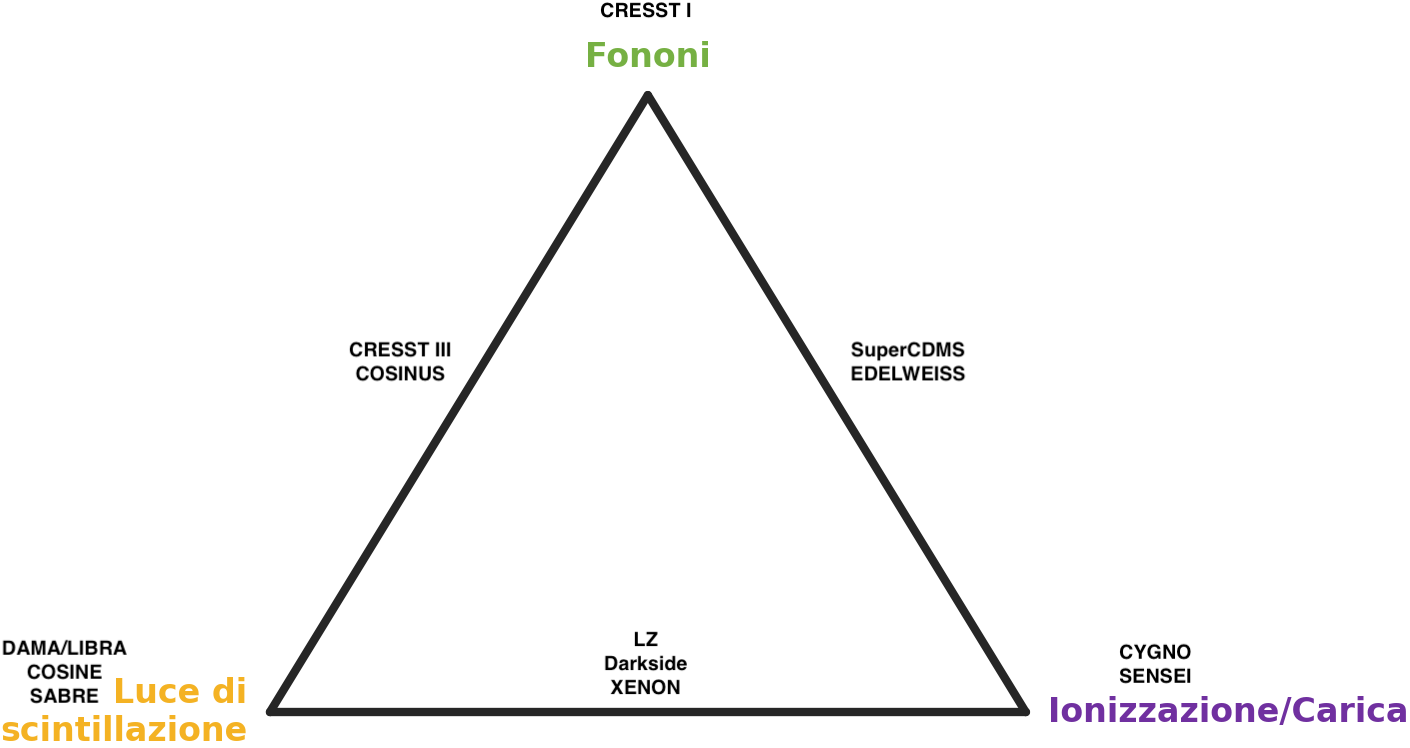
\includegraphics[width=0.8\linewidth]{figures/metodi_DM.png}
    \caption{Rappresentazione schematica dei tre canali di segnale utilizzati nella rivelazione diretta della materia oscura. Gli esperimenti posizionati nelle intersezioni sfruttano la lettura simultanea di due canali per discriminare il fondo radioattivo.}
    \label{fig:approcci}
\end{figure}

\section{Stato dell'arte ed evoluzione delle sensibilità}

In Figura \ref{fig:stato_attuale} è riportato lo stato attuale della ricerca diretta di materia oscura. La regione verde in alto individua lo spazio dei parametri già escluso dai risultati ottenuti. Dal grafico si nota come l'esperimento XENON1T definisca il limite inferiore di sensibilità per WIMP di massa elevata, mentre l'esperimento CRESST III domini la regione delle WIMP a bassa massa grazie all'elevata sensibilità dei rivelatori.

\begin{figure}[htbp]
    \centering
    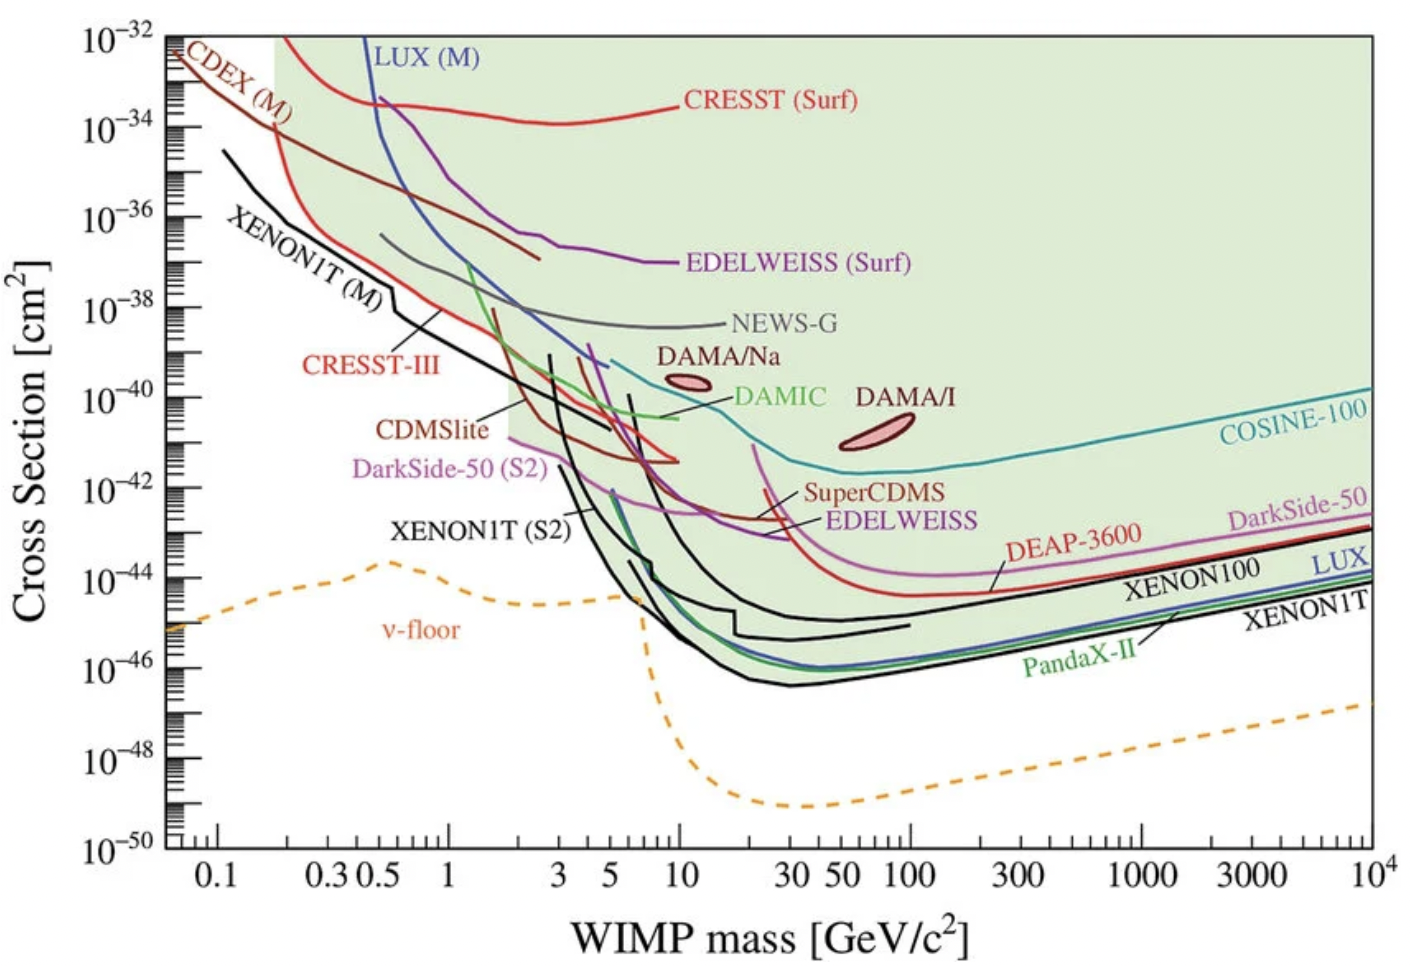
\includegraphics[width=0.8\linewidth]{figures/curva_esclusione_attuale.png}
    \caption{Limiti di esclusione per la sezione d'urto spin-independent WIMP-nucleone. La regione verde rappresenta lo spazio dei parametri escluso dagli esperimenti. Le regioni cerchiate in rosso rappresentano parametri accessibili ottenuti tramite gli esperimenti DAMA/LIBRA, che però non trovano riscontro in esperimenti attuali. Immagine tratta da \cite{Billard2022DirectDM}.}
    \label{fig:stato_attuale}
\end{figure}

Le proiezioni future sono illustrate in Figura \ref{fig:stato_futuro}. È utile notare come la regione verde sia la medesima del grafico precedente, mentre cambiano i valori di sezione d'urto sull'asse verticale. I rivelatori di nuova generazione attualmente in presa dati o in fase di sviluppo in scala di multi-tonnellata (quali XENONnT, LZ e DarkSide-20k) estenderanno ulteriormente la sensibilità, fino a raggiungere il limite intrinseco costituito dalla cosiddetto \textit{neutrino floor}. Parallelamente, per masse inferiori, futuri upgrade di CRESST e altri esperimenti mirati consentiranno di ridurre significativamente lo spazio dei parametri ancora non esplorato.

\begin{figure}[htbp]
    \centering
    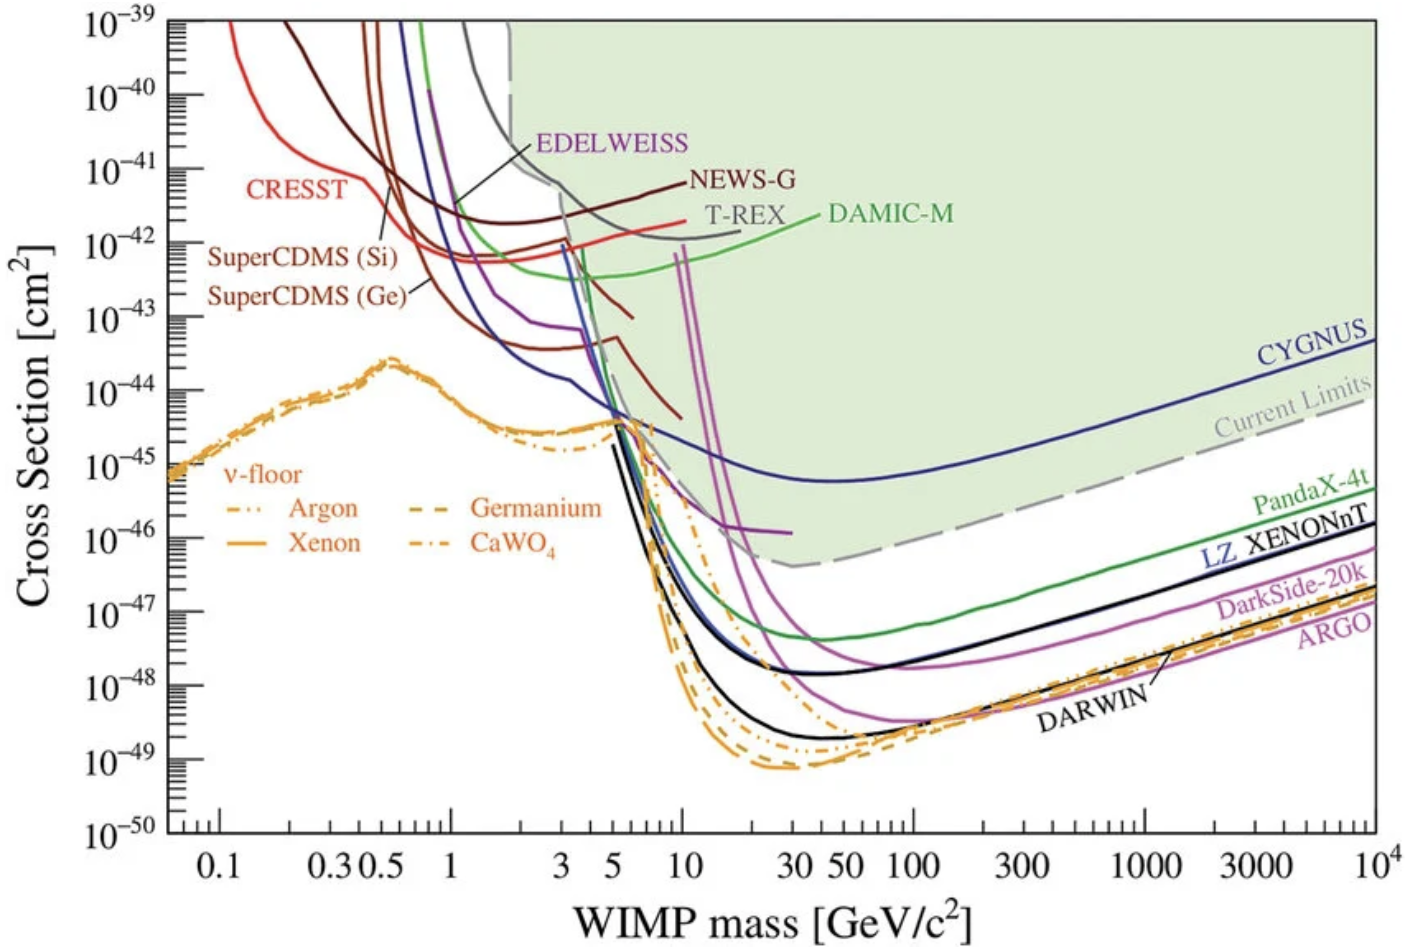
\includegraphics[width=0.8\linewidth]{figures/curva_esclusione_futuro.png}
    \caption{Proiezioni di sensibilità per gli esperimenti di futura generazione. La linea gialla delimita la regione del \textit{neutrino floor}, oltre la quale lo scattering coerente del neutrino costituisce un fondo irriducibile. Le curve inferiori al \textit{Current Limits}, indicano la sensibilità attesa dai futuri esperimenti. Immagine tratta da \cite{Billard2022DirectDM}.}
    \label{fig:stato_futuro}
\end{figure}


